\documentclass[urlcolor=blue,dvipsnames]{beamer}

\usepackage[utf8]{inputenc}
\usepackage{fancybox,fancyvrb}
\usepackage{environ,xspace,empheq}
\usepackage{tikz}
\hypersetup{colorlinks,linkcolor=,urlcolor=cyan}

\beamertemplatenavigationsymbolsempty
\setbeamertemplate{footline}[frame number]
\usetheme{Pittsburgh}

\newcommand\enumnum[1]{{\renewcommand{\insertenumlabel}{#1}%
      \usebeamertemplate{enumerate item} \,}}

\newcommand{\grad}{\nabla}
\newcommand{\ih}{\boldsymbol{\hat{\textbf{\i}}}}
\newcommand{\jh}{\boldsymbol{\hat{\textbf{\j}}}}
\newcommand{\vF}{\boldsymbol{\vec{\textbf{F}}}}
\newcommand{\Matlab}{\textsc{Matlab}\xspace}
\newcommand{\Octave}{\textsc{Octave}\xspace}


\title{9.1 Runge-Kutta methods}

\subtitle{a lesson for MATH F302 Differential Equations}

\author{Ed Bueler, Dept.~of Mathematics and Statistics, UAF}

\date{\tiny \today}


\begin{document}
\setbeamertemplate{itemize item}{$\bullet$}
\setbeamertemplate{itemize subitem}{$\circ$}
\renewcommand{\thefootnote}{{\color{green} \arabic{footnote}}}

\begin{frame}
\titlepage

\centerline{\tiny for textbook: \, D. Zill, \emph{A First Course in Differential Equations with Modeling Applications}, 11th ed.}
%\color{green!40!blue}
\end{frame}


\begin{frame}{the Runge-Kutta happy family}

\begin{itemize}
\item recall improved Euler
\item it is an order 2 method from the \emph{Runge-Kutta} (RK) family
    \begin{itemize}
    \item even Euler itself is an order 1 RK method
    \item there are dozens of useful RK methods of all orders $\ge 1$
    \item $\infty$ly-many methods in the family \dots only a few named
    \end{itemize}
\item these slides describe and test the most-famous RK method, namely \alert{order 4 (classical) RK4}, from about 1900
\item historically, RK4 was accurate enough for most ODE solutions in science and engineering until the 1960s or so
    \begin{itemize}
    \item our \emph{much} better computers and programming languages allow us to reliably debug and use better-than-RK4 methods
    \item \dots which are not intrinsically more accurate, mostly
    \item \dots but they are \emph{adaptive} so the user need not choose step size
    \end{itemize}
\end{itemize}
\end{frame}


\begin{frame}{improved Euler dance}

\begin{itemize}
\item ODE IVP: $\frac{dy}{dt} = t-y^2$, $y(0)=1$
\item show on the direction field: improved Euler with $h=1$
\end{itemize}

\hfill 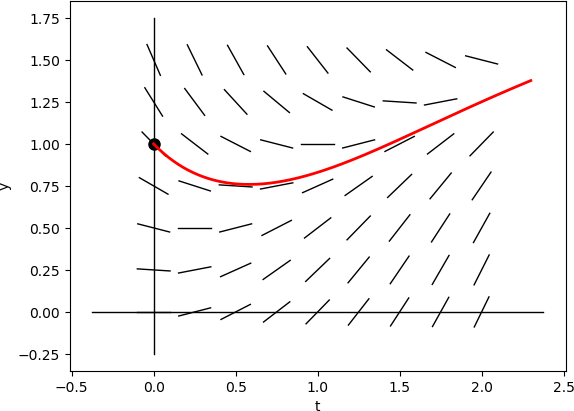
\includegraphics[width=0.8\textwidth]{figs/for-rk4-dir-field}
\end{frame}


\begin{frame}{RK4 dance}

\begin{itemize}
\item ODE IVP: $\frac{dy}{dt} = t-y^2$, $y(0)=1$
\item show on the direction field: RK4 with $h=1$
\end{itemize}

\hfill 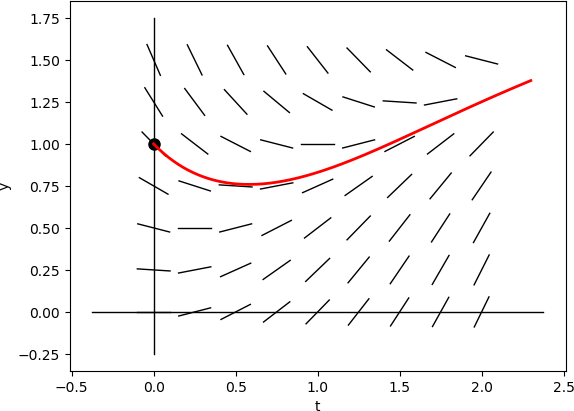
\includegraphics[width=0.8\textwidth]{figs/for-rk4-dir-field}
\end{frame}


\begin{frame}{the RK4 formulas}

\small
\begin{itemize}
\item usually written using four slopes ``$k_i$'' from direction field,
\item and update the $y$-value by a certain average of these slopes:

\vspace{-6mm}
\begin{minipage}[t]{0.4\textwidth}
\begin{align*}
k_1 &= f(t_n,y_n) \\
k_2 &= f(t_n+\frac{h}{2},y_n+\frac{h}{2} k_1) \\
k_3 &= f(t_n+\frac{h}{2},y_n+\frac{h}{2} k_2) \\
k_4 &= f(t_n+h,y_n+h k_3)
\end{align*}
\end{minipage}\begin{minipage}[t]{0.45\textwidth}
\vspace{10mm}

$$\implies y_{n+1} = y_n + h\, \frac{k_1 + 2 k_2 + 2 k_3 + k_4}{6}$$
\end{minipage}
\item here are the formulas for improved Euler, written the same way:

\vspace{-6mm}
\begin{minipage}[t]{0.4\textwidth}
\begin{align*}
k_1 &= f(t_n,y_n) \\
k_2 &= f(t_n+h,y_n+h k_1)
\end{align*}
\end{minipage}
\begin{minipage}[t]{0.4\textwidth}
\vspace{2mm}

$$\implies y_{n+1} = y_n + h\, \frac{k_1 + k_2}{2}$$
\end{minipage}
\item here is Euler itself, written the same way:
$$k_1 = f(t_n,y_n) \qquad \implies y_{n+1} = y_n + h\, k_1$$
\end{itemize}
\end{frame}


\begin{frame}{RK4 scheme in one diagram}

\begin{columns}
\begin{column}{0.35\textwidth}
\small
\begin{itemize}
\item drawing this sketch, or similar, will be an extra credit problem on Midterm 2
\end{itemize}
\end{column}
\begin{column}{0.65\textwidth}
\hfill 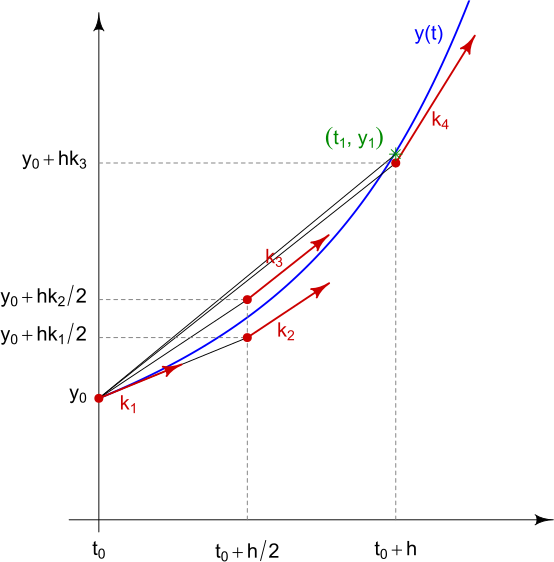
\includegraphics[width=\textwidth]{figs/rk4diagram}
\end{column}
\end{columns}
\end{frame}



\begin{frame}{X}

\begin{itemize}
\item x
\end{itemize}
\end{frame}


\begin{frame}{expectations}

\begin{itemize}
\item just watching this video is \emph{not} enough!
     \begin{itemize}
     \item see ``found online'' videos and stuff at

     \centerline{\href{https://bueler.github.io/math302/week10.html}{\tt \color{cyan} bueler.github.io/math302/week10.html}}
     \item \emph{read} section 9.2 in the textbook
     \item \emph{do} the WebAssign exercises for section 9.2
     \end{itemize}
\end{itemize}
\end{frame}

\end{document}

